\documentclass[../proyecto.tex]{memoir}

\begin{document}

\chapter{Aproximación conceptual}

En este capítulo daremos una descripción conceptual del universo del juego de vida de Conway junto con la del juego de vida de Conway $\alpha$-asíncrono. En este contexto se describe en qué han consistido las simulaciones y sobre qué configuraciones iniciales se han realizado.

\section{Juego de vida de Conway}

Una configuración del juego de vida de Conway es la disposición sobre la malla de un conjunto de nodos ocupados. Por tanto una configuración inicial hace referencia a la disposición inicial de nodos ocupados sobre las que aún no se han aplicado las reglas de evolución. De esta manera cada nodo de la malla tiene dos estados posibles: vacío (0) o  ocupado (1). 

Las reglas de evolución que se aplican en cada iteración simultáneamente a todos los nodos de la malla son las siguientes:
\begin{itemize}
\item Un nodo ocupado se mantiene así si en su vecindario tiene solamente dos o tres nodos ocupados, en otro caso el nodo se vacía.
\item Un nodo vacío se ocupa cuando en su vecindario hay exactamente tres nodos, en otro caso mantiene su estado vacío.
\end{itemize}
Usualmente se consideran como pertenecientes al vecindario los nodos adyacentes en las direcciones horizontal, vertical y diagonales. 

En lo que hemos interpretado como un sentido \textit{biológico}, las reglas se pueden describir también interpretando los nodos ocupados como células vivas y la configuración inicial como una población de células:
\begin{itemize}
\item Una célula puede \textit{morir de soledad}, es decir, tiene solamente una célula en su vecindario o por \textit{superpoblación}, esto es, tiene cuatro o más células en su vecindario.
\item En un nodo vacío \textit{nace} una célula si en su vecindario hay exactamente tres células vivas.
\end{itemize}

La elección de las reglas de evolución parecería \textit{a priori} aleatoria, sin embargo, Conway las escogió aplicando las siguientes pautas \cite{libroGardner}:
\begin{itemize}
	\item No debe existir una disposición inicial de nodos ocupados para la cual haya una \textit{prueba simple} de que la población crezca sin límite. Esto es, no debe de ser posible predecir fácilmente la evolución de una configuración inicial.
	\item Debe haber disposiciones iniciales de nodos ocupados que aparentemente crezcan sin límite. 
	\item Debe haber disposiciones iniciales de nodos ocupados \textit{sencillas} que crezcan y cambien durante un periodo relativamente largo, llegando a tres posibles finales: desaparecer completamente ya sea debido a superpoblación o a dispersión, estabilizarse en una configuración que se mantenga constante o entrar en un ciclo sin fin de oscilación.
\end{itemize}

Sin embargo las reglas que proporcionó Conway no son las únicas que muestran evoluciones interesantes. La siguiente notación nos es útil para expresar distintas reglas de evolución abreviadamente. La reglas de evolución vienen dadas en la forma \textit{Bx/Sy} donde \textit{y} define el número de nodos ocupados en el vecindario para que un nodo ocupado se mantenga y \textit{x} el número de nodos ocupados en el vecindario para que un nodo vacío se ocupe. Por ejemplo, para el juego de vida es B3/S23. Destacamos la regla B1357/S1357 conocida como \textit{Edward Fredkin's replicating automaton}, en la cual cada configuración es eventualmente reemplazada por múltiples copias de sí misma, la regla B3/S12345 conocida como \textit{Maze}, genera configuraciones similares a laberintos, una variación muy curiosa es que si añadimos el número 7 a la parte \textit{B} es posible observar como un nodo ocupado recorre el laberinto y la regla B3/S012345678 conocida como \textit{Life without Death}, en la cual los nodos ocupados nunca se vacían, se caracteriza por un crecimiento caótico y la aparición de configuraciones similares a escaleras que pueden ser usadas para simular circuitos booleanos \cite{regla1}.

%Estaría muy bien añadir imágenes aquí pero me va a tomar un ratete hacerlo.

\subsection{Representación interna y actualización} \label{celulitas}

Como se comentaba en la introducción, plantearse la simulación del juego de vida implica afrontar el problema de representar una malla infinita de dos dimensiones en la memoria finita de un ordenador. Aunque la cantidad de memoria y velocidad de acceso a la misma ha mejorado significativamente con el paso del tiempo, perseguimos una representación que cumpla las siguientes dos características:

\begin{itemize}
\item Una simulación de una configuración inicial del juego de vida tiene que finalizar en un tiempo razonable, pues la clave de los métodos Monte Carlo son la repetición de las mismas y como se comenta posteriormente en \ref{carlino}, al aumentar el número de simulaciones disminuye la varianza, permitiendo mayor precisión.

\item El comportamiento de las configuraciones iniciales es difícil de predecir, por lo que aquellas que crezcan sin límite podrían agotar los recursos de memoria disponibles haciendo que la ejecución sea imposible. En particular, una situación con alto consumo de memoria dificulta la ejecución de múltiples simulaciones independientes en paralelo.
\end{itemize}

Este último punto es, en nuestra opinión, el más restrictivo. Un planteamiento inicial nos podría sugerir que limitar el tamaño de la malla dos dimensional, sin embargo se perdería información en aquellas configuraciones iniciales que excedieran el tamaño fijado de la malla. Para reducir el impacto de la finitud de la malla se ha estudiado la identificación de los bordes opuestos simulando un espacio \textit{infinito} que imita la superficie de un toro, obteniendo resultados favorables \cite{finitudMalla, finitudMalla2}. Pero no es necesario lidiar con los errores derivados de este planteamiento. Una implementación en nuestra opinión más \textit{literal} de la descripción formal del juego de vida, nos permite romper con el paradigma de la limitación de la malla. En lugar de almacenar en memoria la malla completa independientemente de su utilización, se almacenan los nodos ocupados, dados por coordenadas sobre la malla rectangular identificada con el plano cartesiano \cite{boardless}. La contrapartida de esta representación es que los nodos ocupados no son los únicos sobre los que se aplican las reglas, existen nodos vacíos sobre los que también se aplican. Así la implementación del proceso de evolución se puede desglosar en dos etapas:

\begin{itemize}
\item Calcular todos los nodos sobre los que se van a aplicar las reglas de evolución.
\item Aplicar las reglas de evolución sobre cada nodo.
\end{itemize}

El algoritmo de la primera etapa es el siguiente (Algoritmo \ref{alg:pre}). Para cada nodo ocupado se genera su vecindario y en una tabla común a todos los nodos se apunta el número de veces que aparece cada nodo del vecindario. De esta manera en la tabla resultante tenemos enumerados cada nodo que va a evolucionar y el número de nodos ocupados en su vecindario. El vecindario de un nodo ocupado con coordenadas $(x,y)$ viene dado por el conjunto de posiciones que difieren del nodo en cuestión en una unidad como máximo:

\begin{align*}
\begin{array}{lcr}
(x-1,\ y+1) & (x,\ y+1) & (x+1,\ y+1)\\
(x-1,\ y) & (x,\ y) & (x+1,\ y)\\
(x-1,\ y-1) & (x,\ y-1) & (x+1,\ y-1)\\
\end{array} 
\end{align*}


\begin{algorithm}[H]
\caption{Cálculo de los nodos sobre los que se van a aplicar las reglas de evolución}
\label{alg:pre}
\begin{algorithmic}
\REQUIRE $occupiedNodes$ 
\STATE $n \leftarrow [(-1, 1),\ (0, 1),\ (1, 1),\ (-1, 0),\ (1, 0),\ (-1,-1),\ (0,-1),\ (1,-1)]$
\FORALL{$node \in occupiedNodes$}
\FOR{$i=0$ \TO $8$}
\STATE $neighborhoodNode = node + n[i]$
\IF{ $neighborhoodNode \notin table$}
\STATE $table[neighborhoodNode] = 1$
\ELSE
\STATE $table[neighborhoodNode] += 1$
\ENDIF
\ENDFOR
\ENDFOR
\RETURN $table$
\end{algorithmic}
\end{algorithm}

El proceso de evolución de cada nodo almacenado en la variable \textit{table} que devuelve el algoritmo de la etapa anterior se describe en el algoritmo \ref{alg:normal}.

\begin{algorithm}[H]
\caption{Evolución síncrona}
\label{alg:normal}
\begin{algorithmic}
\REQUIRE $table$
\REQUIRE $occupiedNodes$
\STATE $nextOccupiedNodes \leftarrow []$
\FORALL{$node \in table$}
\IF{($table[node] = 3$ \OR $table[node] = 2$) \AND $node\in ocuppiedNodes$}
\STATE $nextOccupiedNodes.append(node)$
\ELSIF{$table[node] = 3$ \AND $node\notin ocuppiedNodes$}
\STATE $nextOccupiedNodes.append(node)$
\ENDIF
\ENDFOR
\RETURN $nextOccupiedNodes$
\end{algorithmic}
\end{algorithm}

Notar que existen algoritmos notablemente más complejos que el descrito en esta sección, como el algoritmo \textit{QuickLife}, el cual se utiliza en una implementación de software libre de un simulador de autómatas celulares llamado \textit{Golly} \cite{quicklife} o el algoritmo \textit{HashLife}. La idea principal de este último algoritmo se basa en el reconocimiento de configuraciones más pequeñas repetidas dentro de la configuración a la que se le están aplicando las reglas de evolución \cite{hashlife}. Nuestra elección viene motivada por la facilidad con la que se puede implementar, describir y modificar para más tarde representar la evolución $\alpha$-asíncrona.

\section{Juego de vida de Conway $\alpha$-asíncrono}

Antes de nada, es importante señalar que la modificación que el juego $\alpha$-asíncrono introduce en las iteraciones de actualización de los estados de los nodos de la malla, sólo afecta a éstos y no a las características de la propia malla.

En un juego de vida $\alpha$-asíncrono cada nodo tiene probabilidad $\alpha$ de ser actualizado y probabilidad $1-\alpha$ de mantener su estado actual. Para ello se ha de generar, para cada nodo, un número pseudo-aleatorio de acuerdo a una distribución uniforme estándar. Si el número obtenido es superior a $\alpha$ las reglas se aplican tal y como están establecidas y, en caso contrario, no se hace, manteniendo el nodo su estado actual. Éste proceso se puede observar en detalle en el algoritmo \ref{alg:async}. Notar que si $\alpha=1$ el algoritmo de actualización $\alpha$-asíncrono coincide con el síncrono.

\begin{algorithm}[H]
\caption{Evolución $\alpha$-síncrona}
\label{alg:async}
\begin{algorithmic}
\REQUIRE $table$
\REQUIRE $occupiedNodes$
\REQUIRE $getRandomNumber()$
\ENSURE  $0 < \alpha \leq 1$
\ENSURE $0< getRandomNumber() < 1$
\STATE $nextOccupiedNodes \leftarrow []$
\FORALL{$node \in table$}
\IF{ $getRandomNumber() < \alpha$ }
\IF{($table[node] = 3$ \OR $table[node] = 2$) \AND $node\in ocuppiedNodes$}
\STATE $nextOccupiedNodes.append(node)$
\ELSIF{$table[node] = 3$ \AND $node\notin ocuppiedNodes$}
\STATE $nextOccupiedNodes.append(node)$
\ENDIF
\ENDIF
\ENDFOR
\RETURN $nextOccupiedNodes$
\end{algorithmic}
\end{algorithm}

\section{Configuraciones iniciales del juego de vida de Conway} \label{zoo}

Como ya se ha indicado anteriormente, en este trabajo tratamos de caracterizar el comportamiento de configuraciones iniciales del juego de vida de Conway bajo la hipótesis de actualización $\alpha$-asíncrona. Nuestra elección de patrones iniciales está motivada por la simplicidad de los mismos, lo que nos permite visualizar de manera sencilla el impacto del $\alpha$-asincronismo.

Dado que las configuraciones iniciales son muy diversas, han existido algunos esfuerzos por realizar una taxonomía de patrones, pero no existe un consenso global. A pesar de ello, hemos considerado la existencia de tres categorías principales que, a continuación, pasamos a describir.

% hay que reestructurar esta parte para que las subcategorías desaparezcan y solo haya tres categorías grandes
\subsection{Vidas inmóviles}
Probablemente las \textit{vidas inmóviles} sean las configuraciones con el comportamiento más simple y fácil de observar. Esta sección está extraída de las siguientes fuentes: \cite{stillLifeProblem},\cite{stillLifeTheory} y \cite{LikeWikiStill}.

Una \textit{vida inmóvil} es una configuración inicial que permanece inalterada en su evolución. A continuación mostramos ejemplos de estos tipos de vidas inmóviles en la \autoref{fig:inmoviles}. La \autoref{fig:2-1} es una \textit{vida inmóvil} en la que todos los nodos ocupados dependen entre sí los unos de los otros, si alguno se queda libre entonces la configuración deja de serlo. Análogamente, en la \autoref{fig:2-2} la mitad horizontal derecha conserva su estabilidad gracias a su homólogo reflejado de la mitad horizontal izquierda y al alterar el estado de cualquier nodo ocupado dicha estabilidad se desvanece. Por último, la \autoref{fig:2-3} es una \textit{vida inmóvil} y a su vez contiene a otra \textit{vida inmóvil}.

\begin{figure}[H]
	\centering
	\begin{subfigure}[b]{0.3\linewidth} 
        \centering
        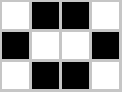
\includegraphics[height=.45\linewidth]{./images/beehive.png}
        \caption{}
        \label{fig:2-1}
    \end{subfigure}
    \quad
	\begin{subfigure}[b]{0.3\linewidth} 
        \centering
        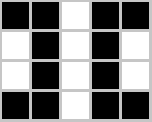
\includegraphics[height=.5\linewidth]{./images/table_on_table.png}
        \caption{}
        \label{fig:2-2}
    \end{subfigure}
	\\    
    \begin{subfigure}[b]{0.3\linewidth} 
        \centering
        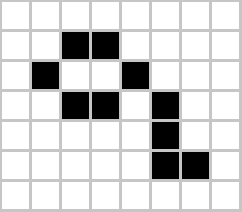
\includegraphics[height=0.5\linewidth]{./images/beehive_with_tail.png}
        \caption{}
        \label{fig:2-3}
    \end{subfigure}
    \quad
	\begin{subfigure}[b]{0.3\linewidth} 
        \centering
        
\includegraphics[height=.35\linewidth]{./images/biblock.png}
        \caption{}
        \label{fig:2-4}
    \end{subfigure}
	\caption{Algunas vidas inmóviles del juego de vida de Conway.}
	\label{fig:inmoviles}
\end{figure} 


Notar que pueden estar formadas a su vez por varias \textit{vida inmóvil} y que o bien dependan entre sí para mantener su estabilidad como en la \autoref{fig:2-3}, o bien sean independientes y al eliminar algunas de ellas la estabilidad se mantenga como en la \autoref{fig:2-4}. También existen \textit{vida inmóvil} que pueden ser separadas en vidas inmóviles independientes y que además existan nodos vacíos que tanto en la configuración inicial como en las \textit{vidas inmóviles} independientes se mantengan así. Un ejemplo de esta situación se pueden observar en \autoref{fig:bimoved}.

\begin{figure}[H]
	\centering
	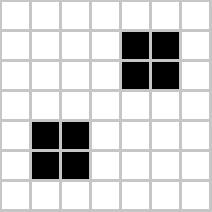
\includegraphics[height=.2\linewidth]{./images/bimoved.png}
	\caption{Configuración inicial que en el centro hay un nodo vacío que se mantiene tanto en las \textit{vidas inmóviles} independientes como en el total.}
	\label{fig:bimoved}
\end{figure} 

Cabría preguntarse el problema de dado un número finito de nodos ocupados, ¿cuántas \textit{vidas inmóviles} diferentes existen? Dicho problema ha sido resuelto para \textit{vidas inmóviles} de hasta 32 nodos ocupados, como se puede consultar en \cite{countStillLifes}.

Por último, hemos observado experimentalmente que las \textit{vidas inmóviles} se mantienen inalteradas también en el juego de vida $\alpha$-asíncrono. Ya que si se actualiza alguno de sus nodos, éste permanece en el mismo estado y si no se actualiza, también. Por tanto podemos concluir que la categoría de \textit{vidas inmóviles} no se ve alterada por la introducción de la evolución $\alpha$-asíncrona. Notar que esto no quiere decir cuando una vida inmóvil colisione con otros tipos de configuraciones se mantenga inalterada. Sin embargo, existen \textit{vidas inmóviles} que cuando colisionan con cierto tipo de naves espaciales generan la destrucción de las mismas y tras algunas iteraciones la configuración vuelve a ser inmóvil. Este tipo de vidas inmóviles se les conoce como \textit{eaters} y existen algunos que mientras que se da la interacción con una configuración, la cual más tarde desaparece, se mantienen en todo el proceso de desaparición inalterados \cite{eater}. 

\subsection{Osciladores}

Un \textit{oscilador} es una configuración inicial que tras un número fijo de iteraciones se repite en la misma posición, al número de iteraciones se le conoce como periodo del \textit{oscilador}. En particular, las vidas inmóviles pueden ser interpretadas como \textit{osciladores} de periodo una iteración.

En la \autoref{fig:congIniciales3} mostramos dos configuraciones iniciales de periodo dos, durante tres iteraciones. Por un lado la \autoref{fig:blinker_evo} muestra tres iteraciones de la configuración inicial nombrada \textit{blinker} y por otro la \autoref{fig:toad_evo} son muestra iteraciones de la configuración inicial \textit{toad}.

\begin{figure}[H]
	\centering
	\begin{subfigure}[b]{\linewidth} 
        \centering
        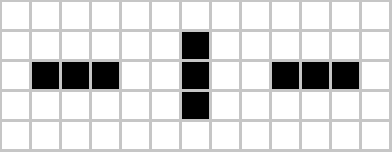
\includegraphics[height=.2\linewidth]{./images/blinker_evo.png}
        \caption{}
        \label{fig:blinker_evo}
    \end{subfigure}
    \\
	\begin{subfigure}[b]{\linewidth} 
        \centering
        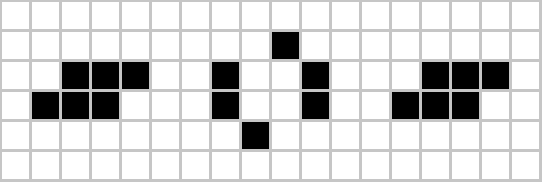
\includegraphics[height=0.2\linewidth]{./images/toad_evo.png}
        \caption{}
        \label{fig:toad_evo}
    \end{subfigure}
	\caption{Primeras 3 iteraciones de 2 \textit{osciladores} de periodo 2 del juego de vida de Conway.}
	\label{fig:congIniciales3}
\end{figure} 

\subsection{Naves espaciales} \label{spaceships}

Una \textit{nave espacial} es una configuración inicial que tras un número fijo de iteraciones se repite pero en una posición desplazada. Particularmente, pueden ser vistas como osciladores que en el periodo de oscilación se desplazan. Dado que este tipo de configuraciones iniciales se desplaza sobre la malla rectangular es interesante considerar la velocidad con la que lo hacen. Si una configuración se desplaza $(dx, dy)$ unidades cada periodo de longitud $n$, la velocidad de desplazamiento de la nave espacial es: $$
 v = \frac{\max\{|dx|,|dy|\}}{k}
$$ 
y su pendiente es $x/y$. Curiosamente se ha probado que para cada pendiente existe una \textit{nave espacial} con dicha pendiente \cite{pendienteNaves}. Notar que $c$ es la velocidad máxima teórica, esto es, un desplazamiento por iteración.

En la \autoref{fig:congIniciales4} encontramos dos \textit{naves espaciales} que se desplazan en distintas direcciones. La \autoref{fig:glider} es la \textit{nave espacial} más pequeña conocida de velocidad $c/4$ y su desplazamiento es diagonal y la \autoref{fig:lightweightspaceship} es la más pequeña conocida de velocidad $c/2$ y su desplazamiento es horizontal.

\begin{figure}[H]
	\centering
	\begin{subfigure}[b]{0.3\linewidth} 
        \centering
        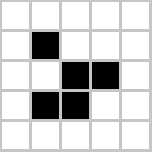
\includegraphics[height=.45\linewidth]{./images/glider.png}
        \caption{}
        \label{fig:glider}
    \end{subfigure}
    \ 
	\begin{subfigure}[b]{0.3\linewidth} 
        \centering
        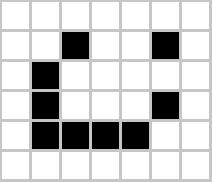
\includegraphics[height=0.45\linewidth]{./images/lightweightspaceship.png}
        \caption{}
        \label{fig:lightweightspaceship}
    \end{subfigure}
	\caption{Dos \textit{naves espaciales} del juego de vida de Conway.}
	\label{fig:congIniciales4}
\end{figure} 

% posibilidad figuras de crecimiento infinito
\subsection{Almacenamiento de las configuraciones iniciales} \label{rle}

Al igual que no existe un consenso global sobre las categorías de configuraciones del juego de vida, tampoco existe una única representación globalmente aceptada para almacenar una configuración en disco. Este problema es similar al de representar una malla rectangular infinita en una memoria finita. Existen soluciones que almacenan el rectángulo más pequeño que contiene a todos los nodos ocupados como sigue: cada fila de este rectángulo esta representada por una cadena de caracteres en la cual los nodos ocupados se identifican por un carácter y los nodos vacíos por otro. Un ejemplo de este tipo de formato es $Life 1.05$ que utiliza el carácter \textbf{*} para los nodos ocupados y el \textbf{.} para los nodos vacíos. 

Sin embargo, este tipo de representación puede ocupar mucho espacio en configuraciones de gran tamaño, por lo que en este trabajo hemos utilizado una versión simplificada del formato \textit{rle} \cite{rle}, el cual es más compacto que el anterior. La primera línea de este formato tiene la forma $x\ =\ m,\ y\ =\ n$ donde m y n son las dimensiones del rectángulo de menor tamaño que contiene a todos los nodos ocupados. La siguiente línea codifica la configuración en una secuencia de elementos de la forma {número de repeticiones}{etiqueta}, donde {número de repeticiones} es el número de ocurrencias de una {etiqueta} que puede ser alguno de los siguientes caracteres: \textbf{b} que representa un nodo vacío, \textbf{o} que representa un nodo ocupado y el carácter \textbf{\$} se emplea para indicar el final de la columna del rectángulo de menor tamaño que contiene a todos los nodos ocupados. El último elemento va seguido del carácter \textbf{!} que indica el final de la configuración. El número de nodos vacíos al final de la última fila de la configuración no tiene que estar necesariamente codificado y tampoco el final de la última fila tiene que incluir al carácter \textbf{\$}. La líneas iniciales de este formato que comiencen por el carácter \# se interpretan como comentarios y por defecto se omiten. Por ejemplo las configuraciones de la \autoref{fig:inmoviles} tendrían la siguiente codificación \textit{rle}:

\begin{itemize}
\item \# Configuración \autoref{fig:2-1} \\
x = 4, y = 3 \\
b2o\$o2bo\$b2o! \\

\item \# Configuración \autoref{fig:2-2} \\
x = 5, y = 4 \\
2ob2o\$bobo\$bobo\$2ob2o!

\item \# Configuración \autoref{fig:2-3} \\
x = 6, y = 5 \\
b2o\$o2bo\$b2obo\$4bo\$4b2o!

\item \# Configuración \autoref{fig:2-4} \\
x = 5, y = 2 \\
2ob2o\$2ob2o!

\end{itemize}

\subsection{Selección de configuraciones iniciales} \label{seleccion}

Los primeros censos de configuraciones iniciales fueron \textit{The Online Life-Life CA Soup Search} y \textit{Achim Flammenkamp's census}, en los que se contabilizaron 174.631.866.050 y 50.158.095.316 configuraciones del juego de vida, respectivamente. El primero de ellos consistió en la evolución de 6.412.048.029 configuraciones iniciales aleatorias que cubren un cuadrado de lado 20 con densidad inicial de 0.5 sobre una malla rectangular infinita \cite{sopa1}. El segundo exploró la evolución de 1.829.196 configuraciones iniciales aleatorias sobre una malla cuadrada de lado 2048 con los bordes opuestos identificados y con una densidad inicial de 0.375 \cite{sopa2}. De ambos censos se puede extraer la conclusión de que las configuraciones que aparecen más a menudo son las \textit{vidas inmóviles}, seguidas por los \textit{osciladores} y por último las \textit{naves espaciales}.


\begin{figure}[H]
	\centering
	\begin{subfigure}[b]{0.3\linewidth} 
        \centering
        
\includegraphics[height=0.45\linewidth]{./images/middleweightspaceship.png}
        \caption{\textit{Middleweight spaceship}}
        \label{fig:middleweightspaceship}
    \end{subfigure}
    \
	\begin{subfigure}[b]{0.3\linewidth} 
        \centering
        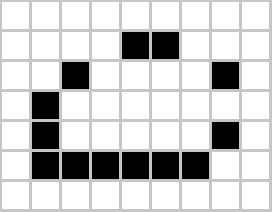
\includegraphics[height=0.45\linewidth]{./images/heavyweightspaceship.png}
        \caption{\textit{Heavyweight spaceship}}
        \label{fig:heavyweightspaceship}
    \end{subfigure}
    \\
	\begin{subfigure}[b]{0.3\linewidth} 
        \centering
        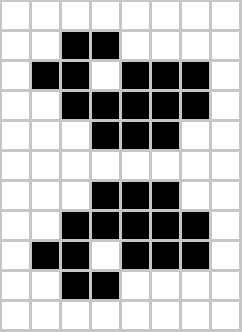
\includegraphics[height=0.65\linewidth]{./images/MWSS_on_MWSS.png}
        \caption{\textit{MWSS on MWSS}}
        \label{fig:mwss2}
    \end{subfigure}
	\caption{Tres últimas \textit{naves espaciales} de las 5 más frecuentes en el censo {Catalogue}.}
	\label{fig:congIniciales5}
\end{figure} 


Para nuestro trabajo tomaremos de referencia el censo más actual \textit{Catalogue} que recoge las ejecuciones de 19.640.649.096.999 configuraciones iniciales aleatorias cuadradas de lado 16 del juego de vida de Conway. Se han obtenido un total de 429.049.899.985.558 patrones de los cuales se encontraron 161.861 tipos diferentes \cite{sopa3}. En la \autoref{tab:sopa1naves} se muestran las primeras 5 \textit{naves espaciales} más frecuentes, de las cuales hemos seleccionado 4 para realizar nuestro experimento. Destacar que todas son de periodo 4 y que no tomaremos más dado que el número de ocurrencias disminuye drásticamente de la cuarta a la quinta posición. En la \autoref{fig:congIniciales5} podemos observar la forma de estas configuraciones iniciales. 

\begin{table}[H]
\centering
\begin{tabular}{|l|l|l|l|}
\hline
\textbf{Nombre}                          & \textbf{Periodo} & \textbf{Ocurrencias}    \\ \hline
\textit{Glider}                 & 4       & 37.699.263.597.381 \\ \hline
\textit{Lightweight spaceship}  & 4       & 55.075.316.989     \\ \hline
\textit{Middleweight spaceship (MWSS)} & 4       & 14.511.262.233      \\ \hline
\textit{Heavyweight spaceship}  & 4       & 2.521.819.486      \\ \hline
\textit{MWSS on MWSS}  & 4       & 7.077      \\ \hline
\end{tabular}
\caption{\textit{Naves espaciales} más frecuentes en el censo {Catalogue}.}
\label{tab:sopa1naves}
\end{table}

Como representantes de la categoría de \textit{osciladores} vamos a estudiar los dos \textit{osciladores} más frecuentes de periodo 2, 3 y 4, cuyas frecuencias se muestran en la \autoref{tab:osciladores}. Los \textit{osciladores} más comunes de periodo 2 son \textit{blinker} y \textit{toad} introducidos anteriormente en la \autoref{fig:congIniciales3}. Los de periodo 3 y 4 son respectivamente \textit{pulsar} y \textit{jam}, y  \textit{mold} y \textit{mazing} (\autoref{fig:toposciladores}).

\begin{figure}[H]
	\centering
	\begin{subfigure}[b]{0.3\linewidth} 
        \centering
        
\includegraphics[height=0.95\linewidth]{./images/pulsar.png}
        \caption{\textit{Pulsar}}
        \label{fig:pulsar}
    \end{subfigure}
    \quad
	\begin{subfigure}[b]{0.3\linewidth} 
        \centering
        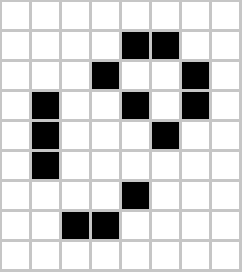
\includegraphics[height=0.7\linewidth]{./images/jam.png}
        \caption{\textit{Jam}}
        \label{fig:jam}
    \end{subfigure}
    \\
	\begin{subfigure}[b]{0.3\linewidth} 
        \centering
        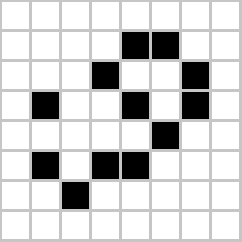
\includegraphics[height=0.65\linewidth]{./images/mold.png}
        \caption{\textit{Mold}}
        \label{fig:mold}
    \end{subfigure}
    \quad
	\begin{subfigure}[b]{0.3\linewidth} 
        \centering
        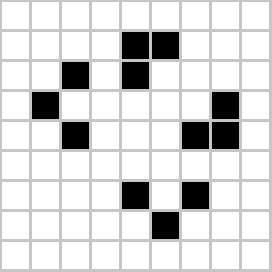
\includegraphics[height=0.65\linewidth]{./images/mazing.png}
        \caption{\textit{Mazing}}
        \label{fig:mazing}
    \end{subfigure}
	\caption{\textit{Osciladores} de periodo 3 y 4 más frecuentes en el censo {Catalogue}.}
	\label{fig:toposciladores}
\end{figure} 


\begin{table}
\centering
\begin{tabular}{|l|l|l|}
\hline
\textbf{Nombre}  & \textbf{Periodo} & \textbf{Ocurrencias} \\ \hline
\textit{Blinker} & 2                & 124.127.579.342.223  \\ \hline
\textit{Toad}    & 2                & 947.040.964.637      \\ \hline
\textit{Pulsar}  & 3                & 30.512.370.641       \\ \hline
\textit{Jam}     & 3                & 676.267              \\ \hline
\textit{Mold}    & 4                & 6.731.991            \\ \hline
\textit{Mazing}  & 4                & 1.281.808            \\ \hline
\end{tabular}
\caption{\textit{Osciladores} de periodos 2, 3 y 4 más frecuentes}
\label{tab:osciladores}
\end{table}

\section{Simulaciones} \label{vars}

Dado el carácter aleatorio del juego de vida $\alpha$-asíncrono emplearemos los fundamentos de Monte Carlo expuestos en la sección \ref{MonteCarlo} para medir los parámetros de interés que a continuación exponemos.

\begin{itemize}
\item Crecimiento de la configuración inicial: dispondremos de tres herramientas para medir el cambio de crecimiento. Estudiaremos la evolución del número de nodos ocupados en cada etapa, la evolución del área del rectángulo de menor tamaño que contenga a todas los nodos ocupados de cada iteración y su densidad, esto es, el cociente del número de nodos ocupados por el área anterior. Cuyas unidades son respectivamente \textit{nodos}, \textit{nodos}$^2$ y \textit{nodos}$^-1$.
\item Tasa de cambio de la configuración inicial: emplearemos el concepto de calor, el número de nodos que cambian de estado por iteración. Cuya unidad es \textit{nodos}.
\item Distribución de los nodos ocupados en cúmulos: contabilizaremos el número de cúmulos por iteración, entendiendo por cúmulo al mayor conjunto de nodos ocupados cuyo vecindario no es disjunto, es decir, en un cúmulo cada nodo ocupado está contenido en el vecindario de otro nodo ocupado del cúmulo.
\item Número de vida inmóviles, esto es, en cada iteración comprobamos cuales de los conjuntos de cúmulos son vidas inmóviles.
\end{itemize}

Estas variables serán medidas para distintos valores de $\alpha$ con el fin de estudiar el efecto de la aleatoriedad en las configuraciones iniciales. 

%\subsection{Descripción algorítmica}

%Esta sección está dedicada a la exposición de los algoritmos que se han diseñado para la extracción de las variables de interés anteriores. Para realizar las simulaciones del juego de vida se ha diseñado una clase, la cual representa el estado interno de un juego de vida $\alpha$-asíncrono, la cual permite evolucionar el

%\subsubsection{Medidas de crecimiento de la configuración inicial}

%La primera herramienta que se comenta para medir el crecimiento de la configuración inicial es el cálculo del número de nodos ocupados en cada etapa. Dado que hemos escogido una representación de la malla en la cual solo se almacenan los nodos ocupados, es suficiente con obtener el tamaño de la estructura de datos en la que se almacena



\subsection{Obtención de los datos}

Dado que realizar múltiples simulaciones de una configuración inicial toma una cantidad considerable de tiempo, hemos considerado la separación del proceso de obtención de datos de las simulaciones en tres etapas bien diferenciadas:
\begin{enumerate}
\item Obtención de las variables de interés para cada conjunto de simulaciones de una configuración inicial.
\item Cálculo de los promedios y sus intervalos de confianza para cada variable en cada iteración.
\item Representación gráfica de los múltiples datos obtenidos para visualizar el impacto de la $\alpha$-asincronicidad en la evolución.
\end{enumerate}

La primera etapa recibe como entrada: \begin{itemize}
\item Número de simulaciones
\item Número de iteraciones que va a realizar cada simulación
\item Distintos valores de $\alpha$ para los que se van a realizar las simulaciones.
\item Una lista de configuraciones iniciales.
\end{itemize}

Con estos datos realiza la ejecución de múltiples simulaciones con un número dijo de iteraciones de una o múltiples configuraciones iniciales. En cada iteración se calcula el número de nodos ocupados, el área del menor rectángulo que contiene a todos ellos, el calor y el número de clústeres. Adicionalmente se calcula un valor que represente unívocamente a una configuración, de manera que en caso de que en la misma iteración de múltiples simulaciones se repita un valor, éste no se almacene por duplicado. Esta etapa genera un archivo en formato \textit{JSON} \cite{json} con las siguientes entradas:

\begin{itemize}
\item \textit{samplerSeed}: dado que cada simulación individual tiene una semilla propia, hemos decidido que dicha semilla sea generada a su vez por otro generador de números pseudo-aleatorios para asegurar una correcta distribución de las mismas. Este campo almacena la semilla que se ha empleado para el generador de semillas, asegurando la reproducibilidad de cada conjunto de simulaciones.
\item \textit{pattern}: este campo almacena el nombre de la configuración inicial sobre la que se han realizado las simulaciones.
\item \textit{alpha}: representa el valor de $\alpha$-asincronismo en la evolución que se ha aplicado las simulaciones, éste valor tiene que estar entre 0 y 1 para ser un valor correcto. En particular, es el valor de $\alpha$ con el que se aplica el algoritmo \ref{alg:async} en cada iteración.
\item \textit{numberOfSteps}: este campo representa el número de iteraciones que se han realizado en cada simulación.
\item \textit{numberOfRuns}: este campo almacena el número de simulaciones que se han realizado.
\item \textit{runs}: es una lista en la cual cada posición corresponde con una iteración, a su vez cada iteración contiene un lista que representa las simulaciones realizadas. Cada elemento de esta última lista tiene las siguientes entradas:
\begin{itemize}
	\item \textit{ncells}: este valor es el número de nodos ocupados.
	\item \textit{nclusters}: este campo es el número de clústeres calculados.
	\item \textit{area}: este valor es el área del menor rectángulo que contiene a todas los nodos ocupados.
	\item \textit{nstillLifes}: este campo contabiliza en número de vidas inmóviles que se han podido localizar.
\end{itemize}
\end{itemize}

%%Añadir un ejemplo JSON

Notar que dado que las simulaciones no comparten información entre sí, pueden ser realizadas en procesos independientes para más tarde agregar todos los resultados en una sola salida.

La siguiente etapa acepta como entrada el archivo en formato JSON de la etapa anterior y calcula el valor medio y de la desviación típica de cada variable, generando un archivo en formato CSV \cite{csv} para cada variable medida en el cual cada fila tiene cuatro columnas en el siguiente orden: número de iteración, media, el radio del intervalo de confianza y el valor de $p-value$ de un test de normalidad (sección \ref{normalidad}). El nombre que recibe cada archivo está compuesto por la variable medida, el valor de $\alpha$, el número de simulaciones y el número de iteraciones. En la etapa final utilizaremos el nombre de los ficheros generados para interpretar su contenido adecuadamente y nombrar a su vez los gráficos de salida. 

Finalmente la última etapa recibe como entrada los archivos CSV generados en la etapa anterior y realiza dos tipos de gráficos. En primer lugar realiza un gráfico para cada archivo de entrada, dónde el eje X viene dado por el número de la iteración, el eje Y por la variable observada, esta última se pinta en conjunción con su intervalo de confianza y el color que representa si supera o no el test de normalidad. A continuación, para cada variable medida realiza un nuevo gráfico, esta vez en lugar de representar la evolución de una variable para un solo valor de $\alpha$, representa la evolución de la variable para todos los valores de $\alpha$. 

%añadir ejemplo gráficas

\end{document}
